\graphicspath{{figs/}} %path to images
\chapter{Implementation (draft)}
\label{ch:lr}
\chaptermark{Fourth Chapter Heading}

\definecolor{codegreen}{rgb}{0,0.6,0}
\definecolor{codegray}{rgb}{0.5,0.5,0.5}
\definecolor{codepurple}{rgb}{0.58,0,0.82}
\definecolor{backcolour}{rgb}{0.95,0.95,0.92}

\lstdefinestyle{mystyle}{
    backgroundcolor=\color{backcolour},
    commentstyle=\color{codegreen},
    keywordstyle=\color{magenta},
    numberstyle=\tiny\color{codegray},
    stringstyle=\color{codepurple},
    basicstyle=\ttfamily\footnotesize,
    breakatwhitespace=false,
    breaklines=true,
    captionpos=b,
    keepspaces=true,
    numbers=left,
    numbersep=5pt,
    showspaces=false,
    showstringspaces=false,
    showtabs=false,
    tabsize=2
}
\lstset{style=mystyle}


The following chapter provides implementation details for the system, including some issues that arose during development and the solutions to these issues.

\section{Component communication}\label{sec:communication}


\section{Entity-Relationship Diagram}

\begin{figure}[t]
    \centering
    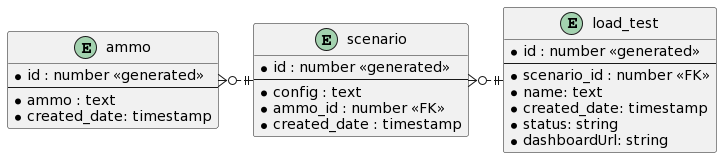
\includegraphics[height=\textheight,width=\textwidth,keepaspectratio]{erl.png}
    \caption{Entity-Relationship Diagram}
    \label{fig:erl}
\end{figure}


\section{Execute test scenario}

\begin{figure}[t]
    \centering
    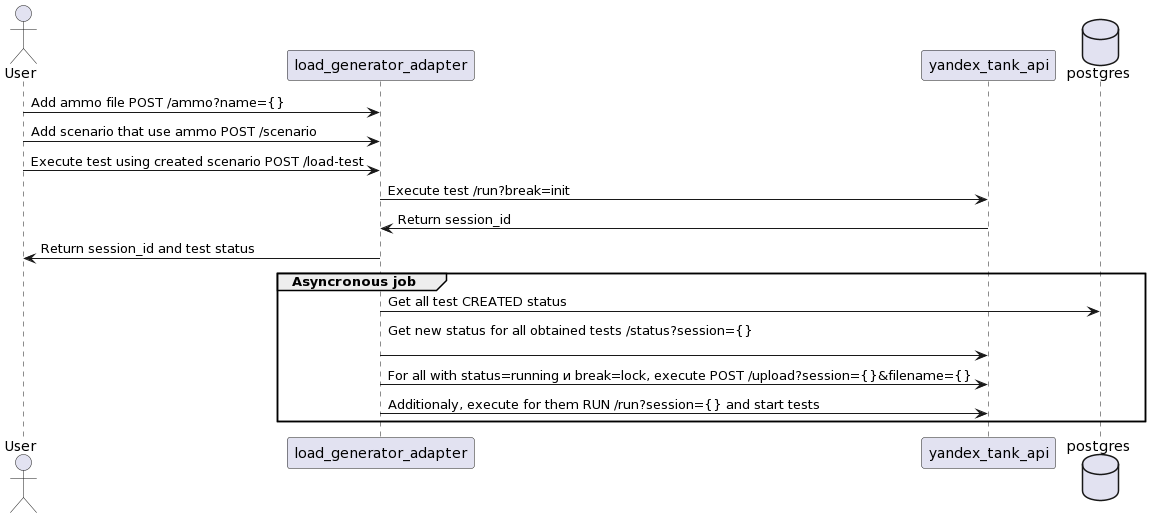
\includegraphics[height=\textheight,width=\textwidth,keepaspectratio]{diagram.png}
    \caption{Execute test scenario}
    \label{fig:test_scenario}
\end{figure}


\lstinputlisting[language=Octave]{code/docker-compose.yaml}